\section{Grafici ed immagini}

\begin{figure}[h]
	\centering
	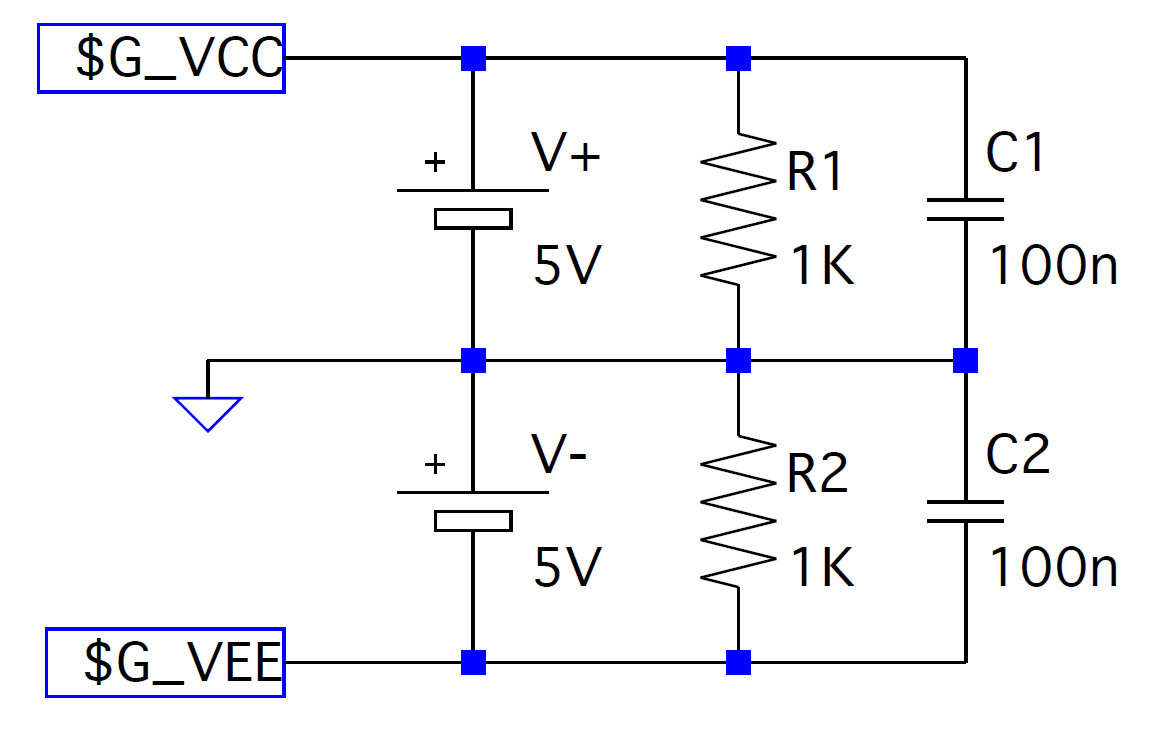
\includegraphics[scale=0.4]{filtraggio.png}
	\caption{Schema del circuito di filtraggio posto all'uscita dell'alimentazione tra 5V e -5V per eliminare eventuali rumori della rete elettrica.}
	\label{f:filtraggio}
\end{figure}

\begin{figure}[h]
	\centering
	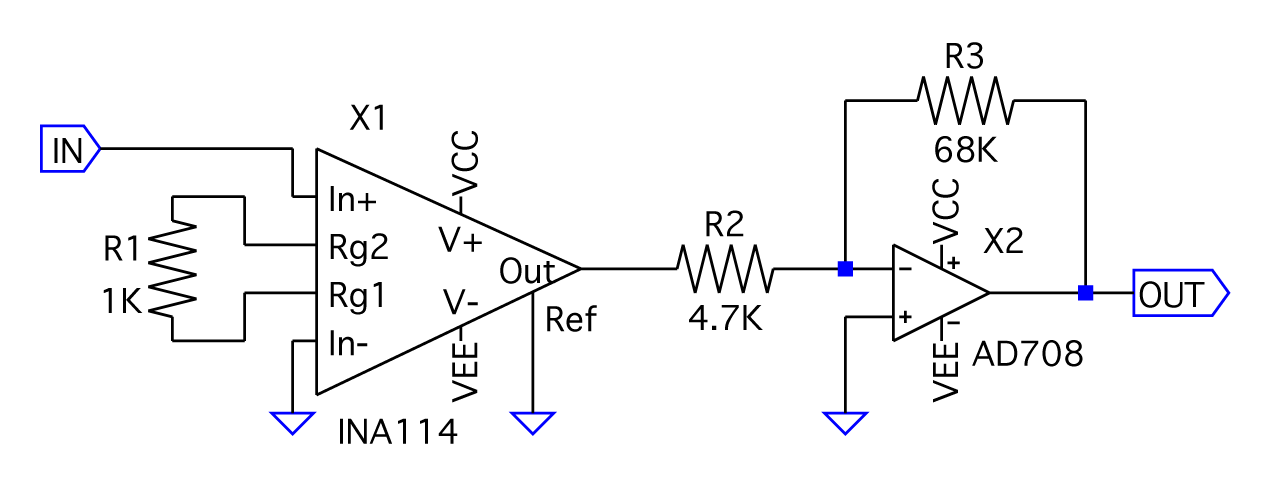
\includegraphics[scale=0.9]{Pre-amp.png}
	\caption{Schema del circuito del pre-amplificatore.}
	\label{f:Pre-amp}
\end{figure}

\begin{figure}[h]
	\centering
	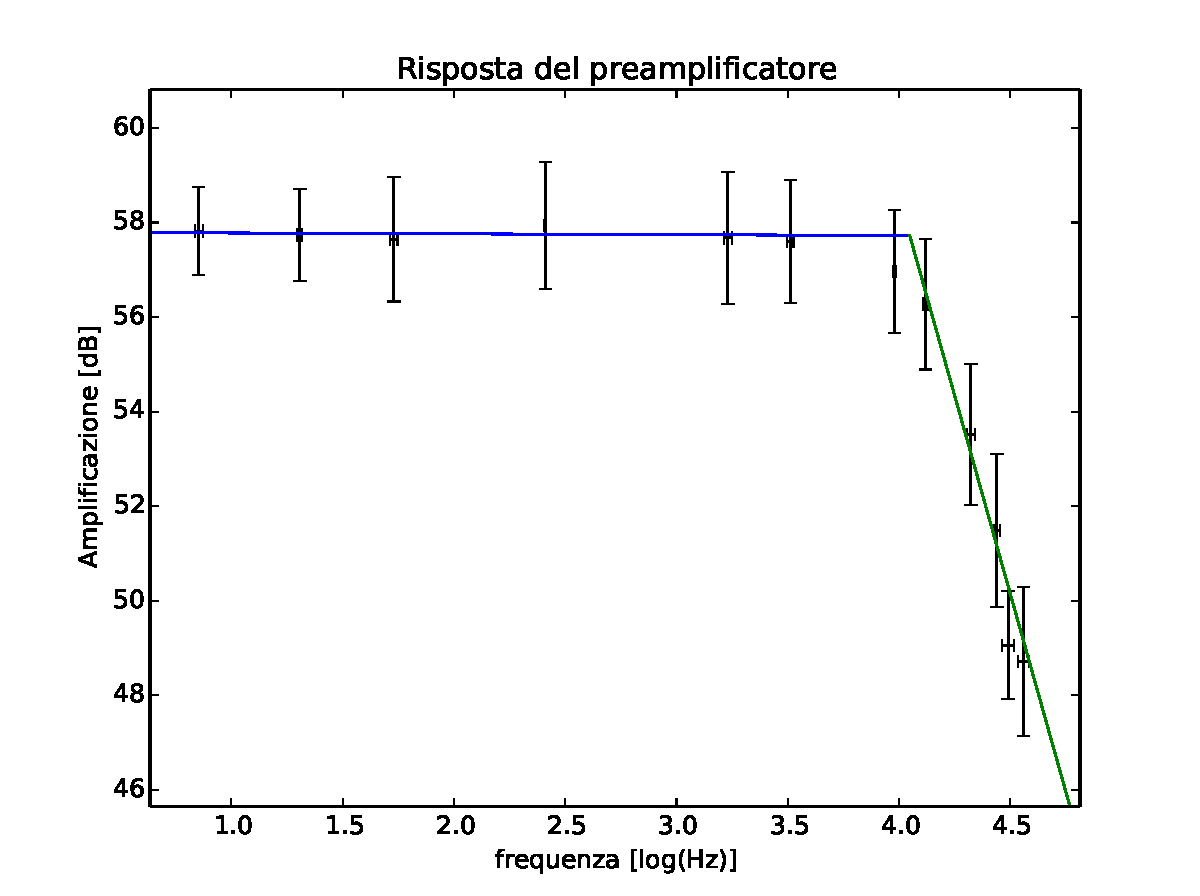
\includegraphics[scale=0.7]{pre-amp.pdf}
	\caption{Plot di Bode per il pre-amplificatore. Sono plottate le rette di fit per le due parti lineari del grafico. Nei fit sono considerate rispettivamente, a partire da sinistra, le prime cinque e le ultime quattro misure.}
	\label{f:pre-amp}
\end{figure}

\begin{figure}[h]
	\centering
	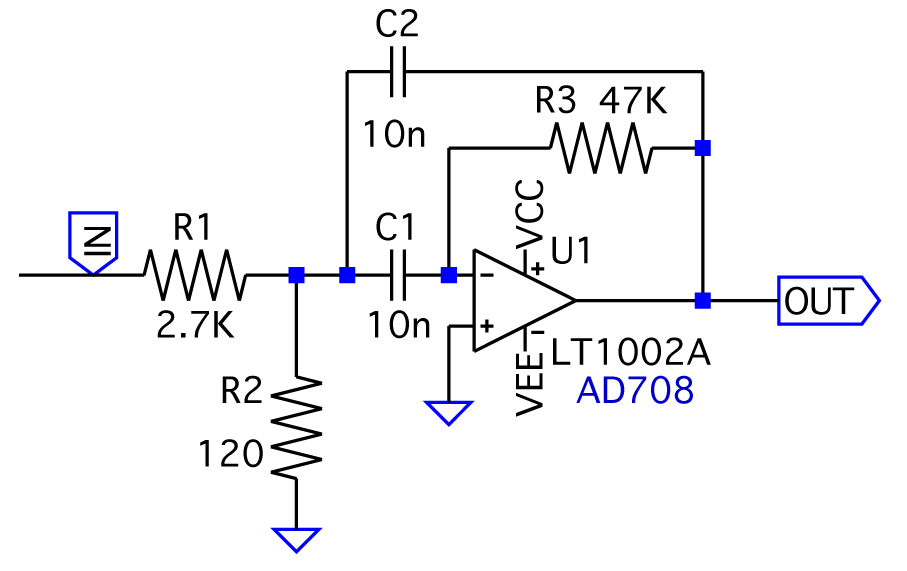
\includegraphics[scale=0.9]{passabanda.png}
	\caption{Schema del circuito del filtro passa-banda.}
	\label{f:passabanda}
\end{figure}

\begin{figure}[h]
	\centering
	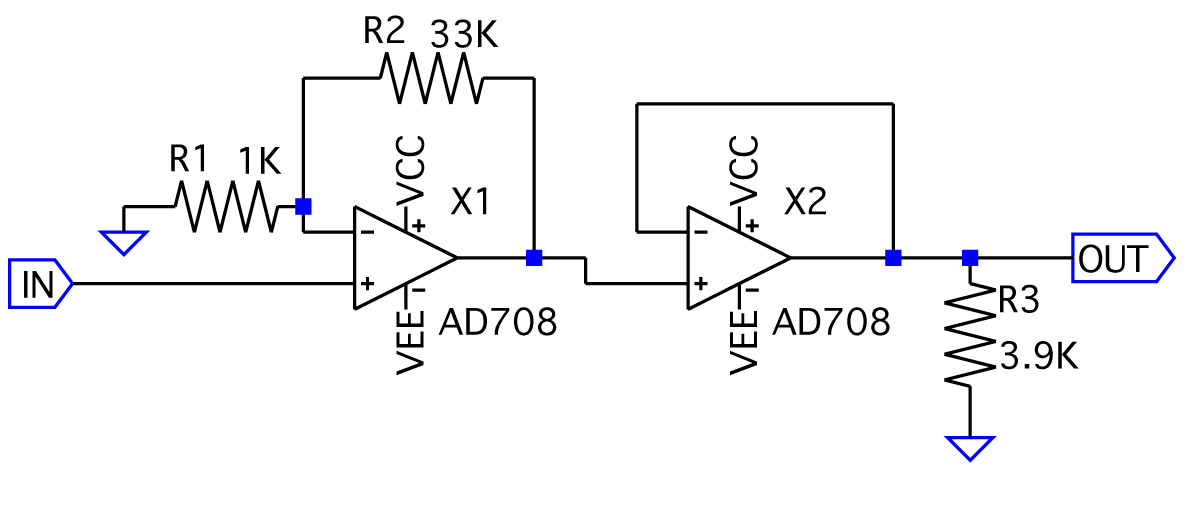
\includegraphics[scale=0.9]{postamp.png}
	\caption{Schema del circuito per il post-amplificatore.}
	\label{f:post-amp}
\end{figure}

\begin{figure}[h]
	\centering
	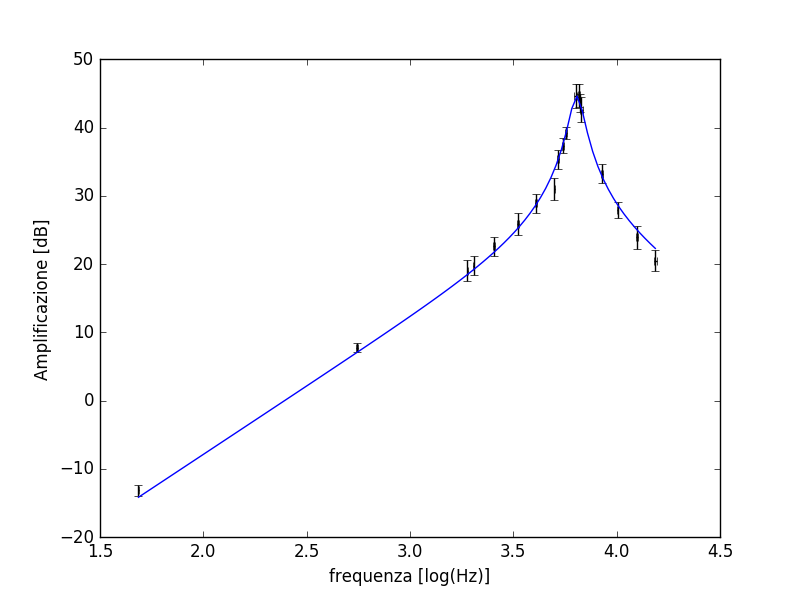
\includegraphics[scale=0.9]{passabanda_fit.png}
	\caption{Fit del modulo della funzione di trasferimento del circuito passa-banda più post-amplificatore.}
	\label{f:passabanda_fit}
\end{figure}

\begin{figure}[h]
	\centering
	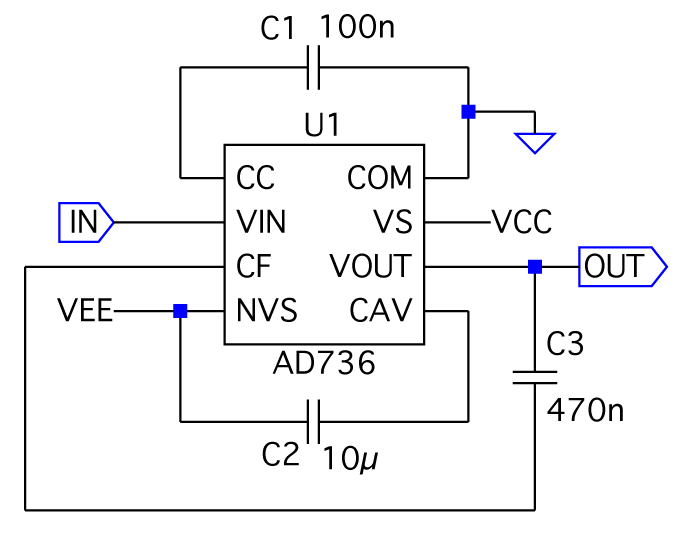
\includegraphics[scale=0.9]{RMS.png}
	\caption{Schema del circuito per il convertitore RMS.}
	\label{f:Convertitore}
\end{figure}

\begin{figure}[h]
	\centering
	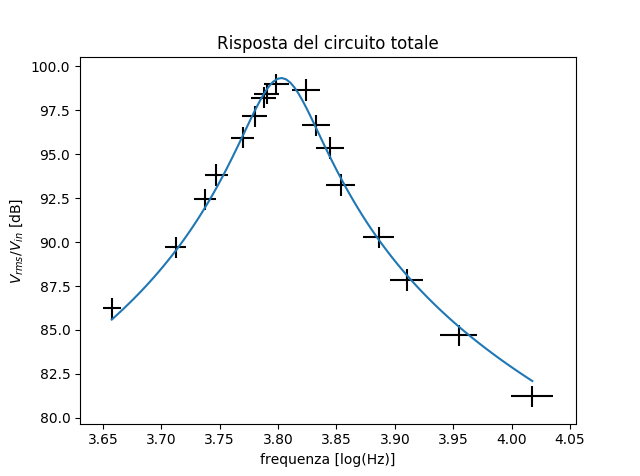
\includegraphics[scale=0.9]{frequenza.png}
	\caption{Risposta in frequenza del circuito completo, con $V_{in}$=18 $\pm$ 5 mV. In ordinate è riportato il rapporto tra il potenziale rms continuo in uscita e l'ampiezza della sinusoide in ingresso}
	\label{f:frequenza}
\end{figure}

\begin{figure}[h]
	\centering
	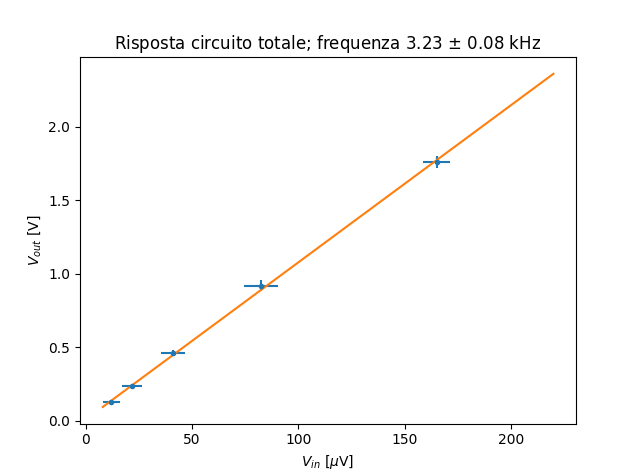
\includegraphics[scale=0.9]{ampiezza.png}
	\caption{Potenziale rms in uscita in funzione dell'ampiezza della sinusoide in ingresso al circuito totale}
	\label{f:risposta_ampiezza}
\end{figure}

\begin{figure}[h]
	\centering
	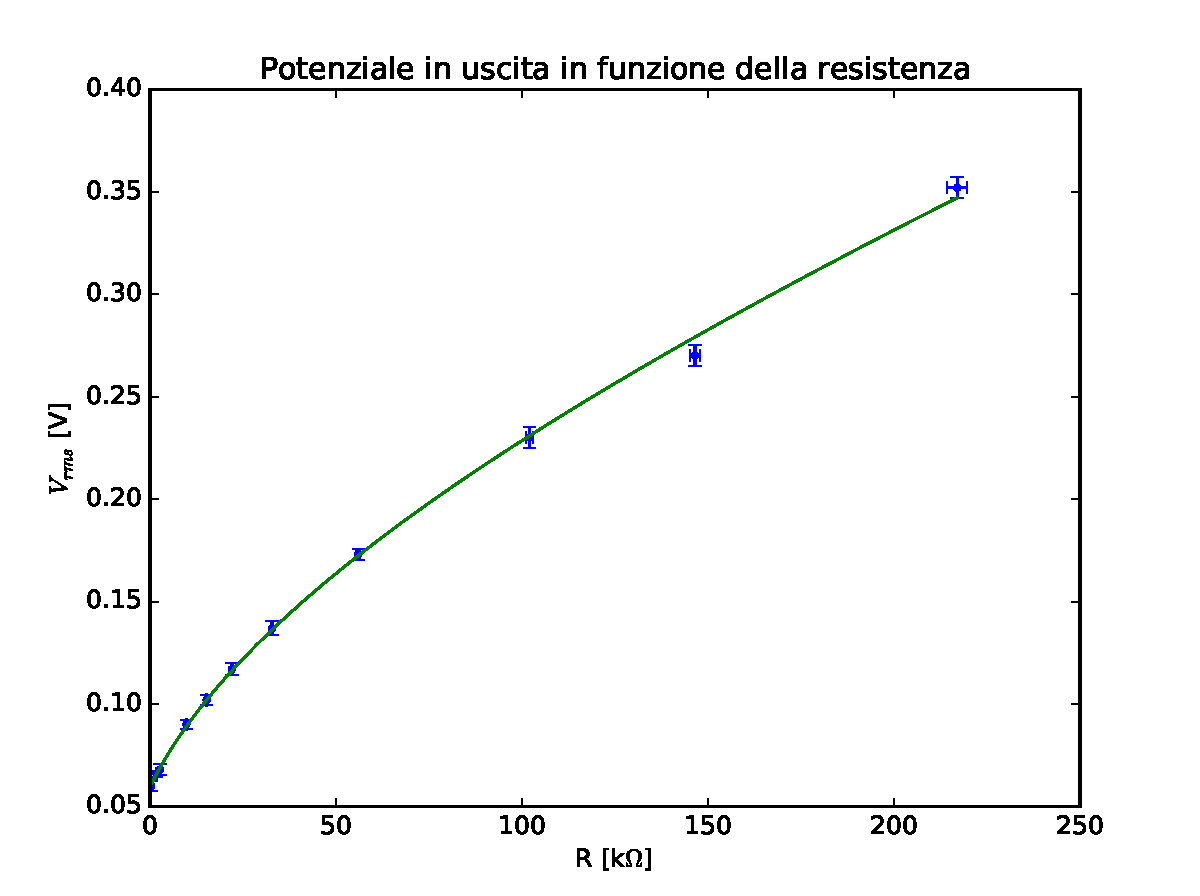
\includegraphics[scale=0.7]{resistenze.pdf}
	\caption{Fit di $V_{RMS}$ in funzione della resistenza in ingresso al circuito completo.}
	\label{f:resistenze}
\end{figure}